\section{Methods}
\label{sec:methods}
In this section, the methods used to compute the magnetic vector potential and the magnetic field
of a straight wire segment and a circular wire loop are established.


\subsection{Straight Wire Segment}


\subsection{Circular Wire Loop}





\subsection{Transformation to Cartesian Coordinates}
Evaluation of the magnetostatic quantites~$A_\varphi$, $B_\rho$ and $B_z$ happens in cylindrical coordinates~$\rho$ and~$z$.
It is often more convenient to be able to work in cartesian coordinates.
Figure~\ref{fig:mappingToCartesian} illustrates the setup of a circular wire loop.
\begin{figure}[htbp]
 \centering
 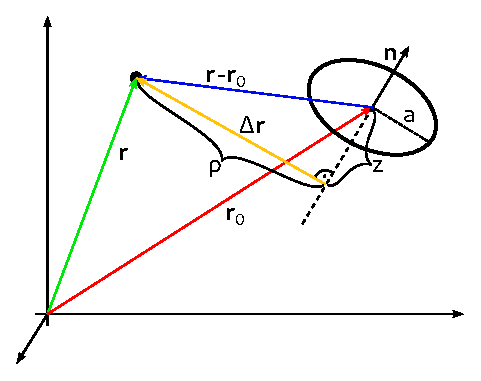
\includegraphics{img/MappingToCartesian.eps}
 \caption{Mapping the components to cartesian coordinates for an exemplatory circular wire loop.
          The loop is centered around its origin~$\mathbf{r}_0$.
          Its normal vector is denoted $\mathbf{n}$ and defines the orientation of the loop.
          The radius of the loop is denoted by~$a$.
          The evaluation location is denoted by~$\mathbf{r}$.}
 \label{fig:mappingToCartesian}
\end{figure}

The $z$-axis of the wire loop's coordinate system is defined by the normal vector~$\mathbf{n}$:
\begin{equation}
  \hat{\mathbf{e}}_z = \frac{\mathbf{n}}{|\mathbf{n}|} \, .
\end{equation}
The $z$ component of the evaluation location is thus obtained as follows:
\begin{equation}
  z = (\mathbf{r} - \mathbf{r}_0) \cdot \hat{\mathbf{e}}_z \, .
\end{equation}
The normalized $z$-coordinate $z'$ is then obtained as:
\begin{equation}
  z' = \frac{1}{a} z = \frac{1}{a} (\mathbf{r} - \mathbf{r}_0) \cdot \hat{\mathbf{e}}_z \, .
\end{equation}
For the radial coordinate, first the vector~$\Delta \mathbf{r}$ is formed:
\begin{equation}
  \Delta \mathbf{r} = (\mathbf{r} - \mathbf{r}_0) - z \, \hat{\mathbf{e}}_z
\end{equation}
and the radial coordinate $\rho$ is then obtained by taking $\rho = |\Delta \mathbf{r}|_2$.
A unit vector in radial direction is formed as follows:
\begin{equation}
  \hat{\mathbf{e}}_\rho = \frac{\Delta \mathbf{r}}{\rho} \, .
\end{equation}
The normalized radial coordinate~$\rho'$ is then obtained as:
\begin{equation}
  \rho' = \frac{1}{a} \rho = \frac{|(\mathbf{r} - \mathbf{r}_0) - z \, \hat{\mathbf{e}}_z|_2}{a} \, .
\end{equation}
The magnetic field of the circular wire loop consists of two cylindrical components, namely $B_\rho$ and $B_z$.
The cartesian magnetic field components are then computed as follows:
\begin{equation}
  \mathbf{B}(\mathbf{r}) = B_\rho \hat{\mathbf{e}}_\rho + B_z \hat{\mathbf{e}}_z \, .
\end{equation}
The magnetic vector potential only has a component in angular direction in the coordinate system of the wire loop.
The corresponding unit vector is $\hat{\mathbf{e}}_\varphi$ with:
\begin{equation}
  \hat{\mathbf{e}}_\varphi = \hat{\mathbf{e}}_\rho \times \hat{\mathbf{e}}_z \, .
\end{equation}
The vector potential of the circular wire loop in thus in cartesian coordinates:
\begin{equation}
  \mathbf{A}(\mathbf{r}) = A_\varphi \hat{\mathbf{e}}_\varphi \, .
\end{equation}

\subsection{Superposition in multi-filament assemblies}
% PolygonFilament
An infinitely thin polygon filament $P$ is described by a list of $N$ points $\mathbf{x}_i$ with $i=1, ..., N$ in three-dimensional (3D) space and a current $I$.
The $(N-1)$ straight connecting lines between each two consecutive points $\mathbf{x}_i$ and $\mathbf{x}_{i+1}$ are assumed to represent the geometry of a wire which carries the current.
If the first and the last point of the polygon filament coincide, the wire forms a closed loop and $\nabla \cdot \mathbf{j} = 0$ is ensured by construction.

The magnetic vector potential $\mathbf{A}(I, \mathbf{x}_i, \mathbf{x}_{i+1}, \mathbf{x})$ and the magnetic field $\mathbf{B}(I, \mathbf{x}_i, \mathbf{x}_{i+1}, \mathbf{x})$
of the wire segments at a location $\mathbf{x}$ can be computed analytically.
The resulting contributions from each segment are superposed in order to compute the resulting magnetic field from the full length of the wire:
\begin{align}
 \mathbf{A}(\mathbf{x}) & = \sum_{i=1}^{N-1} \mathbf{A}(I, \mathbf{x}_i, \mathbf{x}_{i+1}, \mathbf{x}) \quad \mathrm{and} \\
 \mathbf{B}(\mathbf{x}) & = \sum_{i=1}^{N-1} \mathbf{B}(I, \mathbf{x}_i, \mathbf{x}_{i+1}, \mathbf{x}) \quad .
\end{align}
Computationally robust and efficient expressions for
$\mathbf{A}(I, \mathbf{x}_i, \mathbf{x}_{i+1}, \mathbf{x})$ and
$\mathbf{B}(I, \mathbf{x}_i, \mathbf{x}_{i+1}, \mathbf{x})$
are given in Ref.~\cite{hanson_hirshman_2002}.
The detailed derivation of these expressions is given below.

% multi-winding circular coil
